\documentclass{wissdoc}
% ----------------------------------------------------------------
% Hauptdokument
% ----------------------------------------------------------------
%
% Zum Erstellen zweiseitiger PDFs (für Buchdruck) in der Datei "wissdoc.cls" folgende Zeile abändern:
%
% \LoadClass[a4paper,12pt,oneside]{book} % diese Klasse basiert auf ``book''
% in
%\LoadClass[a4paper,12pt,titlepage]{book} % diese Klasse basiert auf ``book''
%
%
% wissdoc Optionen: draft, relaxed, pdf --> siehe wissdoc.cls
% ------------------------------------------------------------------
% Weitere packages: (Dokumentation dazu durch "latex <package>.dtx")
% \usepackage[numbers,sort&compress]{natbib}
\usepackage{csquotes}
\usepackage[backend=biber, style=apa]{biblatex}
\addbibresource{maindoc.bib}

% \usepackage{varioref}
% \usepackage{verbatim}
% \usepackage{float}    %z.B. \floatstyle{ruled}\restylefloat{figure}
% \usepackage{subfigure}
% \usepackage{fancybox} % für schattierte,ovale Boxen etc.
% \usepackage{tabularx} % automatische Spaltenbreite
% \usepackage{supertab} % mehrseitige Tabellen
% \usepackage[svnon,svnfoot]{svnver} % SVN Versionsinformation 
%% ---------------- end of usepackages -------------

%% Informationen für die PDF-Datei
\hypersetup{
 pdfauthor={Felix Thielen},
 pdftitle={(Nested) Named Entity Recognition in deutschen Korpora},
 hidelinks
}

% Macros, nicht unbedingt notwendig
%%%%%%%%%%%%%%%%%%%%%%%%%%%%%%%%%%%%%%%%%%%%%%%%%%%%%%%%%%
% macros.tex -- einige mehr oder weniger nuetzliche Makros
% Autor: Roland Bless 1998
%%%%%%%%%%%%%%%%%%%%%%%%%%%%%%%%%%%%%%%%%%%%%%%%%%%%%%%%%%
% $Id: macros.tex 33 2007-01-23 09:00:59Z bless $
%%%%%%%%%%%%%%%%%%%%%%%%%%%%%%%%%%%%%%%%%%%%%%%%%%%%%%%%%%


%%%%%%%%%%%%%%%%%%%%%%%
% Kommentare 
%%%%%%%%%%%%%%%%%%%%%%%
\ifnotdraftelse{
\newcommand{\Kommentar}[1]{}
}{\newcommand{\Kommentar}[1]{{\em #1}}}
% Alles innerhalb von \Hide{} oder \ignore{} 
% wird von LaTeX komplett ignoriert (wie ein Kommentar)
\newcommand{\Hide}[1]{}
\let\ignore\Hide

%%%%%%%%%%%%%%%%%%%%%%%%%
% Leere Seite ohne Seitennummer, wird aber gezaehlt
%%%%%%%%%%%%%%%%%%%%%%%%%

\newcommand{\leereseite}{% Leerseite ohne Seitennummer, nächste Seite rechts (wenn 2-seitig)
 \clearpage{\pagestyle{empty}\cleardoublepage}
}
%%%%%%%%%%%%%%%%%%%%%%%%%%
% Flattersatz rechts und Silbentrennung, Leerraum nach rechts maximal 1cm
%%%%%%%%%%%%%%%%%%%%%%%%%%
\makeatletter
\newcommand{\myraggedright}{%
 \let\\\@centercr\@rightskip 0pt plus 1cm
 \rightskip\@rightskip
  \leftskip\z@skip
  \parindent\z@
  \spaceskip=.3333em
  \xspaceskip=.5em}
\makeatother

\makeatletter
\newcommand{\mynewline}{%
 \@centercr\@rightskip 0pt plus 1cm
}
\makeatother


%%%%%%%%%%%%%%%%%%%%%%%%%%
% Für Index
%%%%%%%%%%%%%%%%%%%%%%%%%%
\makeatletter
\def\mydotfill{\leavevmode\xleaders\hb@xt@ .44em{\hss.\hss}\hfill\kern\z@}
\makeatother
\def\bold#1{{\bfseries #1}}
\newbox\dbox \setbox\dbox=\hbox to .4em{\hss.\hss} % dot box for leaders
\newskip\rrskipb \rrskipb=.5em plus3em % ragged right space before break
\newskip\rrskipa \rrskipa=-.17em plus -3em minus.11em % ditto, after
\newskip\rlskipa \rlskipa=0pt plus3em % ragged left space after break
\newskip\rlskipb \rlskipb=.33em plus-3em minus.11em % ragged left before break
\newskip\lskip \lskip=3.3\wd\dbox plus1fil minus.3\wd\dbox % for leaders
\newskip \lskipa \lskipa=-2.67em plus -3em minus.11em %after leaders
\mathchardef\rlpen=1000 \mathchardef\leadpen=600
\def\rrspace{\nobreak\hskip\rrskipb\penalty0\hskip\rrskipa}
\def\rlspace{\penalty\rlpen\hskip\rlskipb\vadjust{}\nobreak\hskip\rlskipa}
\let\indexbreak\rlspace
\def\raggedurl{\penalty10000 \hskip.5em plus15em \penalty0 \hskip-.17em plus-15em minus.11em}
\def\raggeditems{\nobreak\hskip\rrskipb \penalty\leadpen \hskip\rrskipa %
\vadjust{}\nobreak\leaders\copy\dbox\hskip\lskip %
\kern3em \penalty\leadpen \hskip\lskipa %
\vadjust{}\nobreak\hskip\rlskipa}
\renewcommand*\see[2]{\rlspace\emph{\seename}~#1} % from makeidx.sty

%%%%%%%%%%%%%%%%%%%%%%%%%%
% Neue Seite rechts, leere linke Seite ohne Headings
%%%%%%%%%%%%%%%%%%%%%%%%%%
\newcommand{\xcleardoublepage}
{{\pagestyle{empty}\cleardoublepage}}

%%%%%%%%%%%%%%%%%%%%%%%%%%
% Tabellenspaltentypen (benoetigt colortbl)
%%%%%%%%%%%%%%%%%%%%%%%%%%
\newcommand{\PBS}[1]{\let\temp=\\#1\let\\=\temp}
\newcolumntype{y}{>{\PBS{\raggedright\hspace{0pt}}}p{1.35cm}}
\newcolumntype{z}{>{\PBS{\raggedright\hspace{0pt}}}p{2.5cm}}
\newcolumntype{q}{>{\PBS{\raggedright\hspace{0pt}}}p{6.5cm}}
\newcolumntype{g}{>{\columncolor[gray]{0.8}}c} % Grau
\newcolumntype{G}{>{\columncolor[gray]{0.9}}c} % helleres Grau

%%%%%%%%%%%%%%%%%%%%%%%%%%
% Anführungszeichen oben und unten
%%%%%%%%%%%%%%%%%%%%%%%%%%
\newcommand{\anf}[1]{"`{#1}"'}

%%%%%%%%%%%%%%%%%%%%%%%%%%
% Tiefstellen von Text
%%%%%%%%%%%%%%%%%%%%%%%%%%
% S\tl{0} setzt die 0 unter das S (ohne Mathemodus!)
% zum Hochstellen gibt es uebrigens \textsuperscript
\makeatletter
\DeclareRobustCommand*\textlowerscript[1]{%
  \@textlowerscript{\selectfont#1}}
\def\@textlowerscript#1{%
  {\m@th\ensuremath{_{\mbox{\fontsize\sf@size\z@#1}}}}}
\let\tl\textlowerscript
\let\ts\textsuperscript
\makeatother

%%%%%%%%%%%%%%%%%%%%%%%%%%
% Gauß-Klammern
%%%%%%%%%%%%%%%%%%%%%%%%%%
\newcommand{\ceil}[1]{\lceil{#1}\rceil}
\newcommand{\floor}[1]{\lfloor{#1}\rfloor}

%%%%%%%%%%%%%%%%%%%%%%%%%%
% Average Operator (analog zu min, max)
%%%%%%%%%%%%%%%%%%%%%%%%%%
\def\avg{\mathop{\mathgroup\symoperators avg}}

%%%%%%%%%%%%%%%%%%%%%%%%%%
% Wortabkürzungen
%%%%%%%%%%%%%%%%%%%%%%%%%%
\def\zB{z.\,B.\ }
\def\dh{d.\,h.\ }
\def\ua{u.\,a.\ }
\def\su{s.\,u.\ }
\newcommand{\bzw}{bzw.\ }

%%%%%%%%%%%%%%%%%%%%%%%%%%%%%%%%%%%
% Einbinden von Graphiken
%%%%%%%%%%%%%%%%%%%%%%%%%%%%%%%%%%%
% global scaling factor
\def\gsf{0.9}
%% Graphik, 
%% 3 Argumente: Datei, Label, Unterschrift
\newcommand{\Abbildung}[3]{%
\begin{figure}[tbh] %
\centerline{\scalebox{\gsf}{\includegraphics*{#1}}} %
\caption{#3} %
\label{#2} %
\end{figure} %
}
\let\Abb\Abbildung
%% Abbps
%% Graphik, skaliert, Angabe der Position
%% 5 Argumente: Position, Breite (0 bis 1.0), Datei, Label, Unterschrift
\newcommand{\Abbildungps}[5]{%
\begin{figure}[#1]%
\begin{center}
\scalebox{\gsf}{\includegraphics*[width=#2\textwidth]{#3}}%
\caption{#5}%
\label{#4}%
\end{center}
\end{figure}%
}
\let\Abbps\Abbildungps
%% Graphik, Angabe der Position, frei wählbares Argument für includegraphics
%% 5 Argumente: Position, Optionen, Datei, Label, Unterschrift
\newcommand{\Abbildungpf}[5]{%
\begin{figure}[#1]%
\begin{center}
\scalebox{\gsf}{\includegraphics*[#2]{#3}}%
\caption{#5}%
\label{#4}%
\end{center}
\end{figure}%
}
\let\Abbpf\Abbildungpf

%%
% Anmerkung: \resizebox{x}{y}{box} skaliert die box auf Breite x und Höhe y,
%            ist x oder y ein !, dann wird das usprüngliche 
%            Seitenverhältnis beibehalten.
%            \rescalebox funktioniert ähnlich, nur das dort ein Faktor
%            statt einer Dimension angegeben wird.
%%
% \Abbps{Position}{Breite in Bruchteilen der Textbreite}{Dateiname}{Label}{Bildunterschrift}
%

\newcommand{\refAbb}[1]{%
s.~Abbildung \ref{#1}}

%%%%%%%%%%%%%%%%%%%%
%% end of macros.tex
%%%%%%%%%%%%%%%%%%%%

% Print URLs not in Typewriter Font
\def\UrlFont{\rm}

\newcommand{\blankpage}{% Leerseite ohne Seitennummer, nächste Seite rechts
 \clearpage{\pagestyle{empty}\cleardoublepage}
}

%% Einstellungen für das gesamte Dokument

% Trennhilfen
% Wichtig! 
% Im ngerman-paket sind zusätzlich folgende Trennhinweise enthalten:
% "- = zusätzliche Trennstelle
% "| = Vermeidung von Ligaturen und mögliche Trennung (bsp: Schaf"|fell)
% "~ = Bindestrich an dem keine Trennung erlaubt ist (bsp: bergauf und "~ab)
% "= = Bindestrich bei dem Worte vor und dahinter getrennt werden dürfen
% "" = Trennstelle ohne Erzeugung eines Trennstrichs (bsp: und/""oder)

% Trennhinweise fuer Woerter hier beschreiben
\hyphenation{
% Pro-to-koll-in-stan-zen
}

% Index-Datei öffnen
\ifnotdraft{\makeindex}

\usepackage{caption}
\captionsetup[table]{skip=1pt}

\begin{document}

\graphicspath{{img/}}

\frontmatter
\pagenumbering{roman}
\ifnotdraft{
 %% titelseite.tex


\def\usesf{}
\let\usesf\sffamily % diese Zeile auskommentieren für normalen TeX Font

\begin{titlepage}
\setlength{\unitlength}{1pt}
\begin{picture}(0,0)(85,770)
%\includegraphics[width=\paperwidth]{logos/KIT_Deckblatt}
\end{picture}

\thispagestyle{empty}

%\begin{titlepage}
%%\let\footnotesize\small \let\footnoterule\relax
\begin{center}
\hbox{}
\vfill
{\usesf
{\huge\bfseries Titel Titel Titel \par}
\vskip 1.8cm
{\huge Seminararbeit / Studienprojekt}\\
\vskip 0.5cm
Untertitel Untertitel Untertitel\ 
\vskip 1.5cm

{\large Universität Trier\\
FB IV - Informatikwissenschaften\\
Lehrstuhl für Wirtschaftsinformatik I\\}

\vskip 3cm
\begin{tabular}{p{3.5cm}l}
Semester: & WiSe/SoSe 20XY \\
Zusatzinfo1: & XYZ XYZ XYZ XYZ (ggf. Betreuer) \\
Zusatzinfo2: & XYZ XYZ XYZ XYZ \\
\end{tabular}
\vskip 3cm
Name(n) und Matrikelnummer(n):\\
\vskip .5cm
Vorname1 Nachname1, Matr.-Nr. 123456\\
Vorname2 Nachname2, Matr.-Nr. 654321\\
Vorname3 Nachname3, Matr.-Nr. 654123\\

}
\end{center}
\vfill
\end{titlepage}


%%% End: 

 %\blankpage % Leerseite auf Titelrückseite

}
%
%% *************** Hier geht's ab ****************
%% ++++++++++++++++++++++++++++++++++++++++++
%% Verzeichnisse
%% ++++++++++++++++++++++++++++++++++++++++++
\ifnotdraft{
{\parskip 0pt\tableofcontents} % toc bitte einzeilig
%\blankpage
% \listoffigures
%\blankpage
\listoftables
%\blankpage
}


%% ++++++++++++++++++++++++++++++++++++++++++
%% Hauptteil
%% ++++++++++++++++++++++++++++++++++++++++++

\mainmatter
\pagenumbering{arabic}
%% einleitung.tex


\chapter{Einleitung}
\label{ch:Einleitung}
%% ==============================

Die Eigennamenerkennung (Named Entity Recognition, im Folgenden NER) ist eine traditionelle Aufgabe der Computerlinguistik mit dem Ziel der Identifikation und Klassifikation von Eigennamen innerhalb eines Textes. Üblicherweise verwendete Klassen sind Personennamen, Ortsnamen und Organisationen, jedoch werden teilweise wesentlich feinere Differenzierungen vorgenommen.

Eine Unteraufgabe der NER ist das Erkennen von verschachtelten Eigennamen (Nested Named Entity Recognition, im Folgenden NNER), also Eigennamen der Form \emph{Universität Trier}, wobei die innere Entität \emph{Trier} gesondert von der äußeren Entität \emph{Universität Trier} ausgezeichnet werden soll. Obwohl verschachtelte Eigennamen sprach- und domänenabhängig einen erheblichen Anteil der Gesamtheit ausmachen können, wird dieser Aufgabe in der Forschung nicht immer eine ebenso erhebliche Bedeutung zugesprochen.

Historisch wurden verschiedene Methoden angewendet, um diese Aufgaben zu lösen. In der modernen Computerlinguistik werden vielerorts neuronale Netze eingesetzt, da sie in vielen Bereichen der Computerlinguistik zu den besten Ergebnissen führen. Eines der meistverwendeten Sprachmodelle, das auch für (N)NER Anwendung findet, ist BERT \parencite{devlin2019bert}.

In \cite{li2019unified} wurde ein einheitliches Framework auf Basis von BERT entwickelt, das für beide Tasks gleichermaßen geeignet sein soll. Da die Ergebnisse vielversprechend sind, aber noch nicht mit deutschen Korpora getestet wurden, wird dies im Rahmen dieser Arbeit nachgeholt. Das Ziel ist, eine erste Einschätzung zu erhalten, ob sich die Ergebnisse von \Citeauthor{li2019unified} auch auf deutsche Korpora übertragen lassen.

% %%% End:
  % Einleitung
%% hauptteil.tex


\chapter{A Unified MRC Framework for NER}
\label{ch:MRC}
%% ==============================


%% ==============================
\section{Überblick}
%% ==============================
\label{ch:MRC:sec:Überblick}

\cite{li2019unified} setzen ihren einheitlichen Ansatz um, indem sie die Aufgaben NER und NNER als Ausprägungen der Machine Reading Comprehension (MRC) interpretieren. Die Problemstellung der Extraktion von Personennamen wird also als eine Frage-Antwort-Aufgabe formuliert, bei der als Antwort auf die Frage \emph{"Welche Person wird im Text erwähnt?"} eine oder mehrere Strecken des Eingabetextes mittels Start- und Endeankern markiert werden, die die Antworten enthalten \parencite[1]{li2019unified}. Analog kann für beliebige weitere Klassen verfahren werden. Als Basis für die Implementierung wird das BERT-Modell \parencite{devlin2019bert} verwendet. Da BERT als Eingabe zwei durch den speziellen [SEP]-Token getrennte Textsequenzen akzeptiert, können Paare aus Frage und Suchtext verwendet werden.

%% ==============================
\section{Anwendung für NER und NNER}
%% ==============================
\label{ch:MRC:sec:AnwendungNERNNER}

Um die Anwendung für (N)NER zu realisieren, werden zwei binäre Klassifikatoren auf den BERT Embeddings trainiert, die für jedes Token des Suchtextes entscheiden, ob es der Start bzw. das Ende einer Antwort im Sinne der formulierten Frage ist \parencite[4]{li2019unified}. Auf diese Weise lässt sich nicht nur einfache NER, sondern auch NNER, sowie die Erkennung möglicherweise überlappender Entitäten umsetzen. Um zuzuordnen, welche Paare aus Anfangs- und Endeanker zusammengehören, wird ein weiterer Klassifikator trainiert, der die dazugehörigen Wahrscheinlichkeiten vorhersagt.

%% ==============================
\section{Datenaufbereitung}
%% ==============================
\label{ch:MRC:sec:Datenaufbereitung}

Oft liegen Trainingsdaten für NER-Anwendungen im BIO-Format oder im CoNLL-Format vor. Für die Zwecke des MRC Frameworks entschieden sich die Autoren für ein Zwischenformat, das ein Tupel aus \textsc{(Frage, Antwort, Kontext)} abbildet \parencite[3]{li2019unified}. Aus diesem Zwischenformat haben die Autoren mittels eines Konversionsscripts die Eingabedaten für ihre angepassten BERT-Datasets erstellt.

Bedauerlicherweise wird das besagte Zwischenformat zwar abstrakt beschrieben, die tatsächliche Implementierung jedoch nicht erklärt. So war es erforderlich, aus dem vorliegenden Quellcode die Funktionsweise zu rekonstruieren und ein zusätzliches Konversionsscript zu programmieren, das aus den deutschen Korpora das benötigte Format herstellt. Das so erzeugte Datenformat ist dargestellt in \autoref{lst:jsonexample}. Jeder Satz wird mittels der Schlüssel \verb|"context"| und \verb|"label"| codiert. Dabei enthält \verb|"context"| den Inhalt des vollständigen Satzes als Whitespace-Verkettung aller Tokens der Eingabedatei. \verb|"label"| enthält als Objekt alle vorhandenen Klassen der Named Entities als Schlüssel. Die Werte dieser Schlüssel sind Listen aus \verb|"<start>;<end>"| Strings, die den Indizes der entsprechenden Vorkommnisse innerhalb des \verb|"context"| entsprechen.

\begin{lstlisting}[caption={Beispiel aus GermEval2014 für das erforderliche JSON-Format}, language={Python}, label={lst:jsonexample}]
	{
		"context": "Aber Borussia Dortmund darf niemals einem allein gehören .",
		"label": {
			"ORG": [
				"1;2"
			],
			"LOC": [
				"2;2"
			]
		}
	}
\end{lstlisting}

Aus den vorhandenen Quelldateien war nicht ersichtlich, ob und wie dieses Format unter Berücksichtigung von NNER angepasst werden muss. Aus diesem Grund wurde die Annahme getroffen, dass eine Verschachtelung wie in \autoref{lst:jsonexample} über die naive Angabe der Indizes bereits ausreichend ist.

%% ==============================
\section{Deutsche Korpora}
%% ==============================
\label{ch:MRC:sec:Deutsche_Korpora}

Die Wahl der Korpora wurde vorrangig durch Verfügbarkeit und Kompatibilität mit dem gegebenen Framework geleitet. Mindestens ein Korpus sollte jedoch NNER abbilden können, weshalb die Entscheidung für GermEval2014 \parencite{germeval2014} getroffen wurde. Mit MultiNERD \parencite{multinerd} wurde ein Korpus betrachtet, das besonders durch die Vielzahl an ausgezeichneten Entity-Klassen interessant ist. Zusätzlich wurde WikiANN \parencite{wikiann} betrachtet, jedoch hauptsächlich aus opportunistischen Gründen bezüglich Verfügbarkeit und Aufwand. Eine Übersicht der verwendeten Korpora ist in \autoref{tab:korpora} dargestellt.

Mit Europeana Newspapers \parencite{europeana} wäre zwar ein weiteres Korpus verfügbar gewesen. Jedoch konnte dieses nicht verwendet werden, da hier keine Trennung der Sätze stattfindet. Der Versuch, mittels Anwendung eines Satztokenizers die Trennung automatisiert vorzunehmen, lieferte keine brauchbaren Ergebnisse. Der Hauptgrund dafür ist vermutlich, dass die Datenquelle dieses Korpus eine OCR-basierte Digitalisierung von Zeitungsartikeln ist, die keine ausreichende Qualität bietet. Dies wird von den Autoren ebenfalls als bestehendes Problem beklagt.

\begin{table}[!htbp]
	\centering
	\caption{Verwendete deutsche Korpora}
	\label{tab:korpora}
	\begin{tabular}{@{}lllll@{}}
		\toprule
		\textbf{Korpus}   & \textbf{Sätze} & \textbf{Tokens}       & \textbf{Nested} & \textbf{Entity-Klassen} \\ \midrule
		GermEval2014    & 31,000         & \textgreater{}590,000 & Ja              & 4                       \\
		WikiANN         & 40,000         & \textgreater{}390,000 & Nein            & 3                       \\
		MultiNERD\footnotemark       & 156,800        & 2,700,000             & Nein            & 15                      \\ \bottomrule
		\end{tabular}
\end{table}
\footnotetext{Die hier gelistete Anzahl der Sätze und Tokens entspricht der Gesamtgröße des Korpus. Zur Verwendung in dieser Arbeit siehe \autoref{ch:Training}.}

%% ==============================
\section{Deutsches BERT-Modell}
%% ==============================
\label{ch:MRC:sec:DeutschBERT}

Während meine früheren Arbeiten auf \verb|bert-german-base-cased| \parencite{bert-base-german-cased} basierten, fiel in dieser Arbeit die Entscheidung für das modernere \verb|gbert-base|, das von \cite{gbert} mit einer deutlich besseren Performance beworben wird. Letztenendes wurde diese Entscheidung aus rein pragmatischen Gründen getroffen, da bereits zu Beginn absehbar war, dass in dieser Arbeit lediglich ein Modell getestet werden kann. Gleichzeitig ist die Wahl des Basismodells nur eine der vielen Stellschrauben, die Einfluss auf die Performance des Frameworks haben. Einige dieser Stellschrauben werden im Folgenden an gegebener Stelle aufgezeigt, sowie in \autoref{ch:Ausblick} überblicksartig zusammengefasst.

%% ==============================
\chapter{Training}
\label{ch:Training}
%% ==============================

%% ==============================
\section{Debugging}
%% ==============================
\label{ch:Training:sec:Debugging}

Im Repository der Autoren befinden sich Scripts, die eine Reproduktion der Ergebnisse aus \cite{li2019unified} ermöglichen sollen. Als Basis für die Anpassung an die deutschen Korpora wurde \verb|scripts/mrc_ner/reproduce/genia.sh| verwendet. Bevor eine angepasste Version dieses Scripts verwendet werden konnte, mussten jedoch zunächst diverse Versionskonflikte der installierten Python-Pakete behoben werden. Dieses Debugging war wie üblich ziemlich zeitaufwändig, da die produzierten Fehlermeldungen nicht immer einen offensichtlichen Hinweis auf das zugrundeliegende Problem lieferten. Die relevanten finalen Versionen der verwendeten Pakete sind in \autoref{lst:packages} aufgeführt. Überraschenderweise zeigen sich große Diskrepanzen zwischen den in dieser Weise ermittelten und den in \verb|requirements.txt| mitgelieferten erforderlichen Versionen.

\begin{lstlisting}[caption={Liste der verwendeten Pakete}, language={Python}, label={lst:packages}]
lightning-utilities==0.9.0
numpy==1.23.5
protobuf==3.20.0
pytorch-lightning==0.9.0
tokenizers==0.13.3
torch==2.0.1
torchmetrics==1.1.0
tqdm==4.66.1
transformers==4.32.0
\end{lstlisting}

Nachdem Konflikte in der Python-Installation bereinigt waren, wurden die in \autoref{ch:MRC:sec:Datenaufbereitung} erläuterten Probleme der Datenformate offenbart. Im Zuge dessen musste das Konversionsscript \verb|conll2json.py| entwickelt werden. Aus den so erhaltenen JSON-Daten wurde mit \verb|ner2mrc/genia2mrc.py| anschließend das benötigte MRC-Format generiert, das letztendlich die Eingabe für das Training darstellt.

Ein weiterer Faktor, der in \autoref{ch:MRC} bereits angedeutet wurde, sind die erforderlichen Formulierungen der Fragen bzw. Queries, anhand derer das Modell Antworten finden soll. Während die einfachste Methode darin besteht, ein einzelnes Wort als Query zu verwenden, kann ebenfalls kurze Umschreibung oder gar eine voll ausformulierte Frage zur Entity-Klasse genutzt werden. Weitere Untersuchungen zu diesem Aspekt finden sich bei \cite[7]{li2019unified}.

Ein erster Versuch, eine mitgelieferte Query-Definition der Autoren unverändert zu übernehmen, ließ das Training zwar erfolgreich abschließen. In der Evaluation wurde jedoch ein enttäuschender F1-Score von ca. 0.51 erreicht. Dies ist auf mangelndes Verständnis des Frameworks zurückzuführen, da beim zweiten Blick offensichtlich wurde, dass die Queries auf Chinesisch formuliert waren.

Ein weiteres Problem zeigte sich beim Versuch, das Modell für MultiNERD zu trainieren. Aufgrund der schieren Größe der Datenmenge (s. \autoref{tab:korpora}) war es nicht machbar, eine Konfiguration der Hyperparameter zu finden, die ein Training auf einer GPU in vertretbarer Zeit ermöglichte. Da die mitgelieferten Reproduktionsscripts ebenfalls Konfigurationen für ein Multi-GPU Setup enthielten, wurde zunächst versucht, diese entsprechend zu übernehmen. Es zeigten sich aber zu große Unterschiede zwischen den Serverarchitekturen der Autoren und dem mir zur Verfügung stehenden Server. Daher wurde der Versuch aufgegeben, das gesamte MultiNERD Korpus zu verwenden. Stattdessen wurde die Größe des Korpus auf \(\frac{1}{6}\) (ca. 26133 Sätze) reduziert, was ein Training auf einer GPU ermöglichte.

Alle finalen Trainings- und Evaluationsscripts können im Anhang eingesehen werden und heißen \verb|germeval_train.sh| bzw. \verb|germeval_eval.sh| und analog für die anderen Korpora.


%% ==============================
\section{Anpassung der Queries}
%% ==============================
\label{ch:Training:sec:Anpassung_Queries}


Die Vorgehensweise in dieser Arbeit folgt aufgrund der Begrenztheit der verfügbaren Zeit und Ressourcen dem in \autoref{tab:queries} dargestellten Ansatz. Die Queries für MultiNERD und WikiANN wurden aus den Definitionen von \cite[4]{multinerd} ins Deutsche übersetzt. Da GermEval2014 der erste für dieses Experiment verwendete Datensatz war, wurden die Ein-Wort-Queries vorläufig nur als Platzhalter eingefügt, um erste plausible Ergebnisse zu erhalten. Da es aber für den Fortschritt des Experimentes wichtiger erschien, zunächst andere Korpora zu untersuchen, wurde auf ein erneutes Training für GermEval2014 mit angepassten Queries verzichtet. Diese Überzeugung wurde außerdem dadurch gefestigt, dass es sich bei der fortschreitenden Arbeit zeigte, dass die Länge der Queries erheblichen Einfluss auf den Ressourcenbedarf des Trainings hat: Das Training mit vollständigen Definitionen erfordert ca. 50\% mehr Zeit und VRAM als das Training mit Ein-Wort-Queries. In Anbetracht der ohnehin erheblichen Trainingsdauer (vgl. \autoref{tab:evaluation}) wurde daher auf wiederholtes Training mit angepassten Queries und/oder Hyperparametern verzichtet.

\begin{table}[!htbp]
	\centering
	\caption{Art der Queries für die Korpora}
	\label{tab:queries}
	\begin{tabular}{@{}ll@{}}
	\toprule
		\textbf{Korpus} & \textbf{Query Defintionen} \\ \midrule
		GermEval2014    & Ein-Wort-Query             \\
		WikiANN         & Übersetzte Definitionen aus MultiNERD \\
		MultiNERD       & Übersetzte Definitionen aus MultiNERD \\ \bottomrule
	\end{tabular}
\end{table}

%% ==============================
\chapter{Evaluation}
\label{ch:Evaluation}
%% ==============================

%% ==============================
\section{Übersicht der Trainingsergebnisse}
%% ==============================
\label{ch:Evaluation:sec:Übersicht_der_Trainingsergebnisse}

Es folgen in \autoref{tab:evaluation} die Ergebnisse der Evaluation des MRC-Frameworks. Insgesamt sind die Ergebnisse vergleichbar mit den englischsprachigen Korpora von \cite[6]{li2019unified}. Speziell die mit MultiNERD erreichten Scores übertreffen diese teilweise sogar deutlich. Auch wenn die Performance auf GermEval2014 ungefähr 6\%\textendash8\% schlechter abschneidet, sind die Ergebnisse wesentlich besser als die ursprünglichen Systeme der GermEval Konferenz \parencite[6]{germeval2014}. Außerdem sind sie vergleichbar mit moderneren Modellen wie \cite[3,4]{riedl-pado-shootout}, die auf diesem Korpus trainiert wurden. Für das deutsche WikiANN gibt es kaum Vergleichswerte, jedoch wird von \cite{Schiesser_2023} ein etwas besserer F1-Score von 0.8892 berichtet.

Die Evaluation fand mit den zur Verfügung stehenden Skripten der Autoren statt. Metriken werden als Span-level micro-average berichtet \parencite[5,6]{li2019unified}.

\begin{table}[!htbp]
	\centering
	\caption{Evaluation des MRC-Frameworks}
	\label{tab:evaluation}
	\resizebox{\columnwidth}{!}{
		\begin{tabular}{@{}l|ccc|ccc|c@{}}
		\specialrule{.1em}{0em}{0em}
		\textbf{Korpus}       & \multicolumn{3}{c|}{\textbf{dev}}                       & \multicolumn{3}{c|}{\textbf{test}}                  & \textbf{Trainingsdauer}                         \\
		\textbf{} & \textbf{f1}     & \textbf{precision} & \textbf{recall} & \textbf{f1} & \textbf{precision} & \textbf{recall} & \multicolumn{1}{c}{\textbf{(in Min.)}} \\
		\specialrule{.05em}{0em}{0em}
		GermEval2014    & 0.8255          & 0.8379             & 0.8136          & 0.8111          & 0.8369             & 0.7867          & 200                               \\
		WikiANN         & 0.8578          & 0.8625             & 0.8532          & 0.8604          & 0.8545             & 0.8665          & 223                               \\
		MultiNERD       & \textbf{0.8823} & \textbf{0.8986}    & \textbf{0.8665} & \textbf{0.8841} & \textbf{0.8994}    & \textbf{0.8692} & 644                               \\ \specialrule{.1em}{0em}{0em}
		\end{tabular}
	}
\end{table}

%% ==============================
\section{Interpretation der Trainingsergebnisse}
%% ==============================
\label{ch:Evaluation:sec:Interpretation_der_Trainingsergebnisse}

Es gibt verschiedene Erklärungsansätze für die Beobachtung, dass GermEval2014 deutlich schlechter abschneidet als die anderen Korpora. Einerseits ist GermEval2014 der einzige Datensatz des NNER-Tasks, was möglicherweise dazu führt, dass die Evaluation bspw. das Nichterkennen einer inneren Entity bestraft, obwohl die äußere Entity korrekt erkannt wurde. Diese Schwierigkeit fällt bei reiner NER nicht ins Gewicht. Zudem ist GermEval2014 auch das deutlich kleinste Korpus (vgl. \autoref{tab:korpora}), wodurch möglicherweise kein ausreichendes Training möglich war. Außerdem war es, wie in \autoref{ch:Training:sec:Anpassung_Queries} beschrieben, das erste Korpus, auf dem trainiert wurde, und hatte lediglich Ein-Wort-Queries als Basis. Es ist mit Sicherheit davon auszugehen, dass dieser Faktor die Performance entscheidend reduziert hat.

WikiANN und MultiNERD sind maschinell generierte silver-standard Korpora. Das führt zu einer großen Menge an Trainingsdaten, die jedoch nicht immer von hoher Qualität sind. Demzufolge ist die Qualität eines trainierten Modells nicht notwendigerweise besonders gut, obwohl die Evaluation dieses Modells positiv ausfällt.

Infolgedessen sind die Ergebnisse in dieser Form nur eingeschränkt vergleichbar. Um ein tatsächlich faires Bild der Performance des MRC\--Frame-work-s zu erhalten, sollten weitere Experimente durchgeführt werden. Mögliche Faktoren, die dabei berücksichtigt werden könnten, werden in \autoref{ch:Ausblick} aufgeführt.

%% ==============================
\chapter{Ausblick}
%% ==============================
\label{ch:Ausblick}

Trotz der aufschlussreichen Ergebnisse bezüglich der Performance des MRC\--Frame\-work\-s auf deutschen Korpora gibt es an vielen Stellen Bedarf für weitere Untersuchungen. Im Rahmen dieser Arbeit war vor allem angesichts der hohen Trainingsdauer nicht möglich, auf alle denkbaren Konfigurationen einzugehen. Im Folgenden werden einige Aspekte aufgeführt werden, von denen zu erwarten ist, dass sie großen Einfluss auf die Performance des Frameworks haben.

\begin{itemize}
	\item \textbf{Hyperparameter:} Die Anzahl der Epochen, die Batch-Size und die Lernrate sind offensichtliche Hyperparameter, mit denen experimentiert werden könnte. Mögliche Versuche sind allerdings direkt gebunden an die verfügbaren Ressourcen.
	\item \textbf{Queries:} Wie in \autoref{ch:Training:sec:Anpassung_Queries} beschrieben, ist die Formulierung der Queries ein entscheidender Faktor, der von \cite{li2019unified} genauer beleuchtet wurde. Allerdings wurde nicht im Speziellen die deutsche Sprache diskutiert. Obwohl zu vermuten ist, dass sich die Beobachtungen der Autoren auch auf das Deutsche übertragen lassen, bleibt dies zu überprüfen.
	\item \textbf{Korpora:} Da die in dieser Arbeit gewählten Korpora lediglich eine kleine Auswahl der verfügbaren Daten darstellen, ist es naheliegend, die Untersuchungen auf weitere Korpora auszubreiten, sowie eine technische Konfiguration zu erreichen, in der ein Training mit dem vollständigen MultiNERD Korpus möglich ist.
	\item \textbf{BERT-Modell:} Das verwendete Modell \verb|gbert-base| wirkt zwar vielversprechend, trotzdem ist es denkbar, dass andere Modelle, die bspw. auf BERT\textsubscript{LARGE} oder RoBERTa basieren, bessere Ergebnisse liefern. Eine andere Modellarchitektur, die überhaupt nicht auf BERT basiert, ist zwar theoretisch denkbar. Da jedoch das gesamte MRC\--Frame\-work auf die BERT-Architektur ausgelegt ist, wäre dies nicht ohne erheblichen Aufwand umsetzbar.
\end{itemize}

   % Hauptteil
%% schluss.tex


\chapter{Fazit}
\label{ch:Fazit}
%% ==============================

Hier könnte Ihr Fazit stehen.

%%% End: 
     % Schluss



%% ++++++++++++++++++++++++++++++++++++++++++
%% Anhang
%% ++++++++++++++++++++++++++++++++++++++++++

\appendix
% %% ==============================
% \section{Anhang}
% %% ==============================
% \label{app:conll2json.py}

% \lstinputlisting[language=python]{src/python/conll2json.py}

%\include{anhang_a}
%\include{anhang_b}

%% ++++++++++++++++++++++++++++++++++++++++++
%% Literatur
%% ++++++++++++++++++++++++++++++++++++++++++
%  mit dem Befehl \nocite werden auch nicht 
%  zitierte Referenzen abgedruckt

\cleardoublepage
\phantomsection
\addcontentsline{toc}{chapter}{\bibname}
%%
% \nocite{*} % nur angeben, wenn auch nicht im Text zitierte Quellen 
           % erscheinen sollen
% \bibliographystyle{itmabbrv} % mit abgekürzten Vornamen der Autoren
%\bibliographystyle{gerplain} % abbrvnat unsrtnat
% spezielle Zitierstile: Labels mit vier Buchstaben und Jahreszahl
%\bibliographystyle{itmalpha}  % ausgeschriebene Vornamen der Autoren
% \bibliography{maindoc}

% Redefine the plain page style to have an empty header
\fancypagestyle{plain}{
  \fancyhf{} % clear all header and footer fields
  \fancyfoot[R]{\thepage} % Page number centered at the bottom
  \renewcommand{\headrulewidth}{0.5pt} % no head rule
  \renewcommand{\footrulewidth}{0pt} % no foot rule
}

% Use the plain page style for the bibliography
\pagestyle{plain}
\printbibliography % Print the bibliography

%% ++++++++++++++++++++++++++++++++++++++++++
%% Index
%% ++++++++++++++++++++++++++++++++++++++++++
\ifnotdraft{
\cleardoublepage
\phantomsection
\printindex            % Index, Stichwortverzeichnis
}

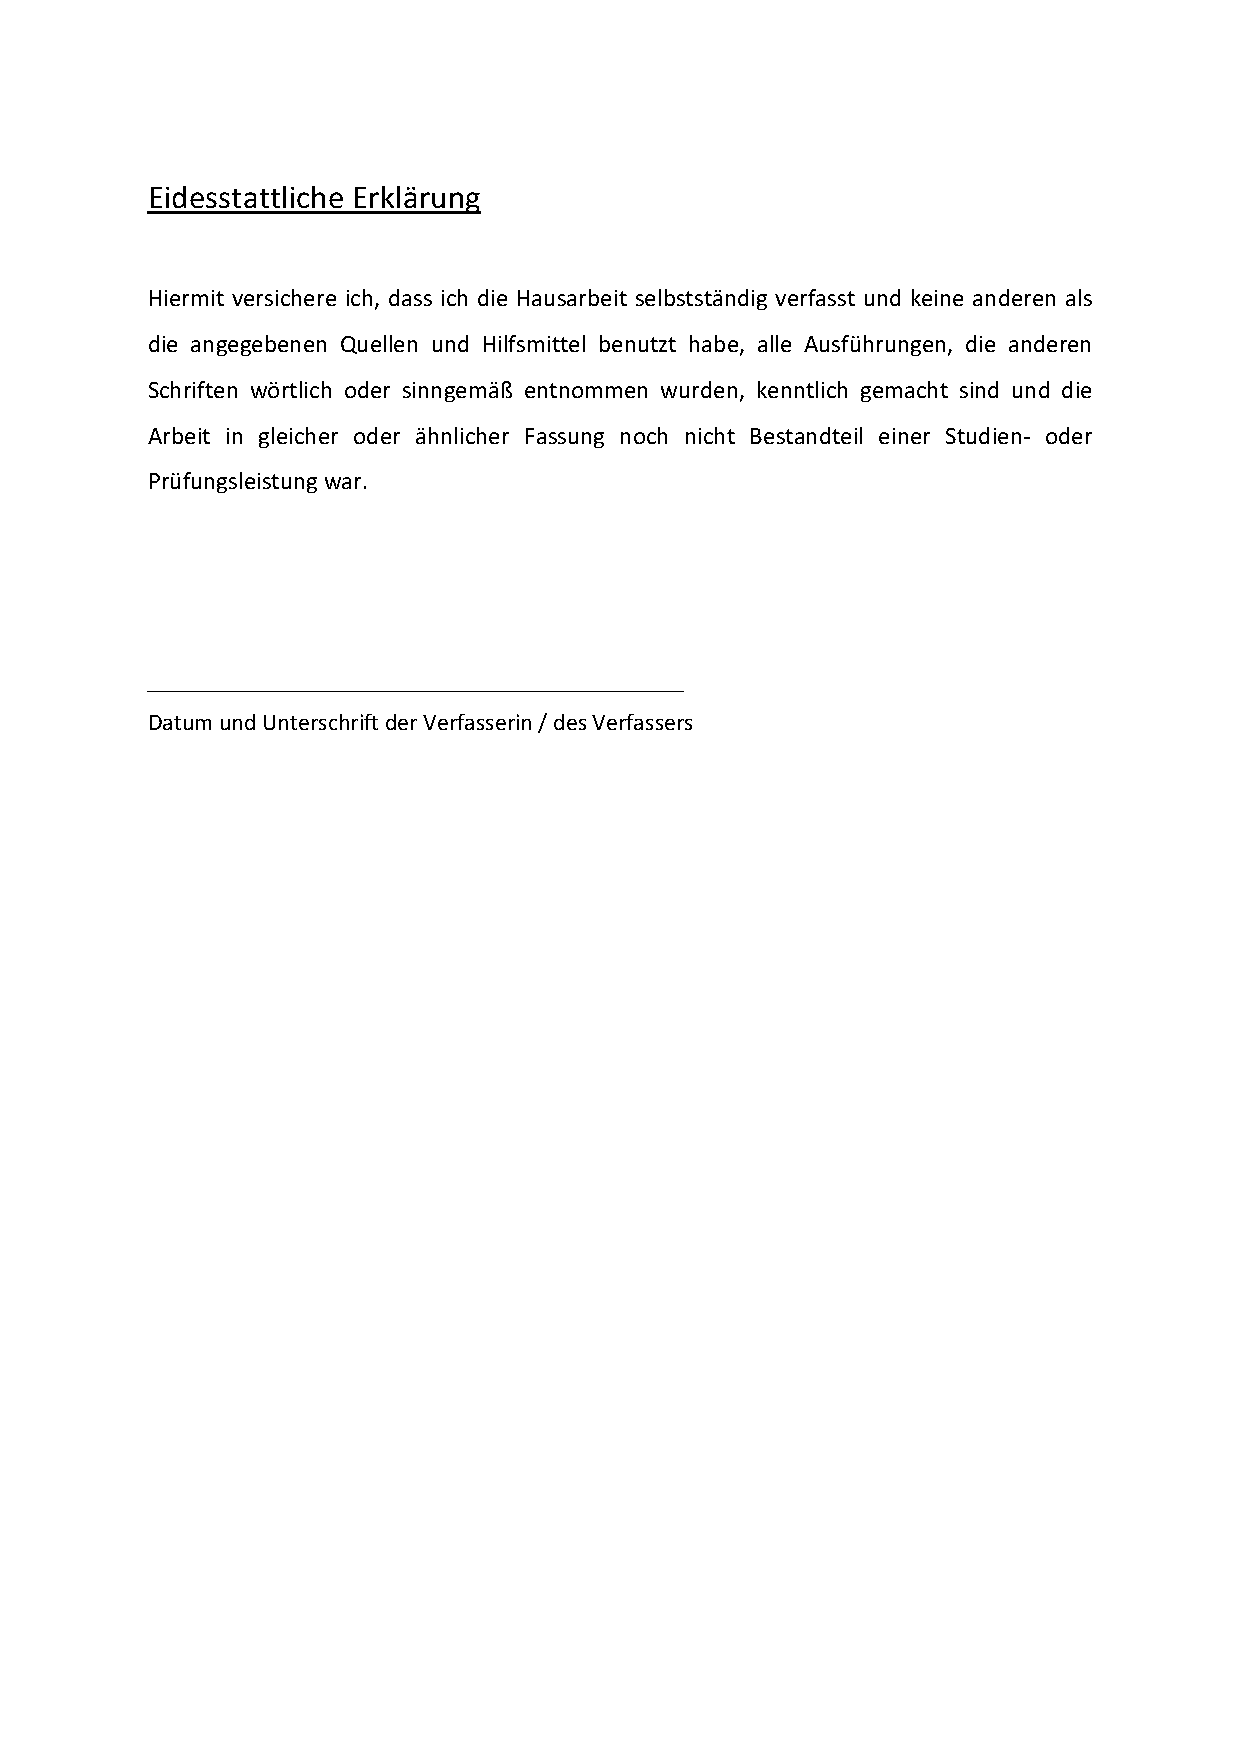
\includepdf[pages=-]{img/plagiatserklaerung.pdf}

\blankpage % Leerseite 
 
\end{document}
%% end of file
